% Generated mechanically from docs/paper-full-draft-v6-evaluation-hierarchy.md.
% Scientific content remains synchronized with that evaluation-hierarchy Markdown manuscript.
\documentclass[sigconf,nonacm]{acmart}

%%% do not modify the following VLDB block %%
%%% VLDB block start %%%
\usepackage{pvldb}
%%% VLDB block end %%%

\usepackage{array}
\usepackage{tabularx}
\renewcommand\vldbdoi{XX.XX/XXX.XX}
\renewcommand\vldbpages{XXX-XXX}
\renewcommand\vldbavailabilityurl{https://github.com/1951123/ce-replay}

\begin{document}
\title{CE-Replay: Executable Cardinality-Estimation Semantics for Statistics Physical Design}

% AUTHOR METADATA PENDING: replace these explicit placeholders before submission.
\author{AUTHOR METADATA PENDING}
\affiliation{%
  \institution{AFFILIATION METADATA PENDING}
  \city{CITY METADATA PENDING}
  \country{COUNTRY METADATA PENDING}
}
\email{EMAIL-METADATA-PENDING@example.invalid}

\begin{abstract}
Selecting extended statistics for a supplied target workload is a physical-design problem with two distinct constraints: statistics can interact non-monotonically through the estimator, and deployed objects consume recurring maintenance capacity. Independent candidate scores are therefore insufficient because native applicability, winner selection, clause consumption, and mechanism composition make each candidate's effect contextual. We introduce CE-Replay, a workload-specialized, design-parametric representation that keeps the supported statistics-sensitive estimator semantics executable and exposes both an objective oracle and a semantic dependency oracle. We instantiate CE-Replay for PostgreSQL 16.14 conjunctive base-relation restrictions with MCV, functional-dependency, and constant \texttt{IN}/\texttt{= ANY} MCV semantics, and use it with deterministic maintenance-constrained local search. Across sparse Census and dense IN-heavy DMV, CE-Replay matches fresh native PostgreSQL estimates on 468/468 and 1,965/1,965 queries, supports mixed-mechanism designs, and preserves audited incremental move decisions while reducing semantic replay work; the mixed evaluator also shows that less semantic work need not yield lower wall-clock time. These results establish that executable native semantics can support statistics physical design within a validated fragment, while broader CE coverage, hypothetical-payload acquisition, realization-robust selection, and runtime objectives remain open.
\end{abstract}
\maketitle

%%% do not modify the following VLDB block %%
%%% VLDB block start %%%
\vldbtopmatter
%%% VLDB block end %%%

\section{Introduction}\label{sec:1}

Cost-based query optimization depends on estimates of how many tuples flow through candidate plans. Ordinary per-column statistics can be inadequate when predicates are correlated, so DBMSs provide extended statistics that expose multivariate information to the estimator. Deciding which extended statistics to maintain changes the information available during optimization and is therefore a physical-design decision, not merely a statistics-collection setting. This paper studies that decision for a supplied target workload.

Selection is semantically necessary because a DBMS may choose among overlapping statistics, consume clauses after using one statistic, compose statistics over disjoint dimensions, and suppress a downstream mechanism after an upstream mechanism changes the residual state. A candidate's effect therefore depends on the other selected objects and their physical realization. In both Census and DMV, some additions worsen the target-workload cardinality-estimation objective; even with loose capacity, selecting every statistic is not a valid default in these settings.

Selection also has an independent resource justification. PostgreSQL must collect and refresh deployed statistics, and this recurring \texttt{ANALYZE} work depends on the mechanism and environment. A practical design must balance estimator utility against maintenance capacity: a statistic may be affordable yet harmful, or beneficial yet infeasible.

Automatic statistics management already considers dependencies among statistics, while physical-design research establishes contextual interactions among design objects; what-if interfaces and reusable configuration-parametric optimizer representations are also established ~\cite{chaudhuri2001statistics,schnaitter2009interactions,chaudhuri1998whatif,papadomanolakis2007inum,bruno2008cpqo}. Dependency-aware exact recomputation is likewise a general and database precedent ~\cite{liu2016incremental}. The challenge addressed here is narrower: preserve the native estimator state transitions through which a statistics design changes applicability, clause consumption, numerical contribution, and downstream mechanism reachability, then use that state both for hypothetical CE and statistics-semantic move invalidation.

Our key idea is to specialize the DBMS's supported statistics-sensitive estimator semantics to the supplied workload while leaving statistics-design-dependent behavior executable. Workload-fixed clauses, relation context, and ordinary selectivities become fixed context; candidate payloads remain explicit inputs; and applicability, winner selection, clause consumption, mechanism composition, and numerical updates execute for each hypothetical design. The result, CE-Replay, produces the DBMS-style cardinality estimate. Ground truth enters only at the design layer, where the estimate is converted into q-error and a workload objective.

Executable semantics provide two interfaces. The \textbf{objective oracle} evaluates the estimate and loss induced by a hypothetical physical statistics state without learning a separate subset-to-q-error response model inside the supported fragment. The \textbf{dependency oracle} identifies the queries, semantic dimensions, and downstream mechanisms that a design move can affect. Because both interfaces arise from the same executable state transitions, the optimizer can avoid semantically irrelevant recomputation while preserving audited move values.

We instantiate CE-Replay for the supported PostgreSQL 16.14 statistics-sensitive fragment of conjunctive base-relation restrictions. The implementation covers validated scalar predicates, constant \texttt{IN} and \texttt{= ANY} MCV predicates, multicolumn most-common-values statistics, functional dependencies, PostgreSQL precedence relevant to MCV ties, and directed MCV-to-FD composition. It is source-informed and validated against native instrumentation; it is not a complete PostgreSQL CE emulator or an automatic source compiler.

We evaluate two structurally contrasting workloads: Census has a large candidate universe with sparse candidate-query incidence, while DMV has a small, dense, high-reuse universe dominated by constant \texttt{IN} predicates. Within the supported realization boundary, replay matches native raw estimates to floating-point tolerance, including all 468 fresh Census queries and all 1,965 fresh DMV queries after deployment. The experiments establish non-monotone utility, mechanism-dependent maintenance cost, mixed MCV+FD selection, and audited incremental equivalence. The evidence does not make the workloads representative, the workload-scale search globally optimal, or reduced semantic work a guarantee of lower runtime.

This paper makes four contributions:

\begin{enumerate}
\item \textbf{Problem and representation.} We formulate statistics design under a maintenance constraint over the supported native CE state transitions. Applicability, consumption, precedence, and downstream reachability remain executable design semantics. The formulation separates selected definitions, DBMS-specific physical realization, frozen payloads, and fresh realization.
\item \textbf{PostgreSQL CE-Replay.} We implement and validate CE-Replay for the supported PostgreSQL 16.14 base-restriction MCV+FD fragment, including bounded constant ScalarArray semantics and directed mechanism composition. The scope is explicit and excludes arbitrary PostgreSQL CE.
\item \textbf{Semantics-guided optimization.} We use CE-Replay as a validated objective oracle and a statistics-semantic dependency oracle for deterministic maintenance-constrained ADD/DROP/SWAP search, including incremental move evaluation that reproduces audited full-replay move values within the supported setting. Workload-scale guarantees are neighborhood-local rather than global.
\item \textbf{Cross-workload physical validation.} We demonstrate contextual non-monotonicity, maintenance-aware mixed designs, dependency-aware evaluation, and fresh physical deployment on sparse Census and dense IN-heavy DMV. The evidence concerns CE loss and semantic fidelity, not query-runtime improvement.
\end{enumerate}
\section{Background and Motivation}\label{sec:2}

\subsection{Extended statistics and cardinality estimation}

A query optimizer estimates predicate selectivity and intermediate cardinality to compare candidate plans. Per-column statistics commonly induce an independence approximation for multiple predicates; correlations can make that approximation inaccurate. Work on correlation discovery and multivariate summaries addresses this gap, and PostgreSQL exposes functional-dependency and MCV extended statistics for selected attribute groups ~\cite{ilyas2004cords,postgresql16docs}.

PostgreSQL supports several extended-statistics mechanisms. The two used here have different semantics. A multicolumn MCV object stores frequent value combinations and frequencies, allowing compatible predicates to be tested directly against a joint distribution. A functional-dependency object records approximate dependency strengths and adjusts the treatment of equality-eligible predicates. Section 4 describes only the control and numerical behavior required by CE-Replay.

\subsection{Statistics as physical design}

A candidate statistic specifies a persistent definition that may be deployed and refreshed. Unlike an index, it does not primarily add an access operator; it changes the estimator's information state and hence the estimates used during plan search. Workload-aware statistics management, selective statistics collection, and resource-constrained physical design are established research areas ~\cite{chaudhuri2001statistics,elhelw2007jits,bruno2008constrained}. The selected design studied here additionally depends on native statistics-consumption semantics and recurring maintenance work.

Candidate definition, payload, and realization are distinct. A definition identifies what PostgreSQL should collect; a payload contains sampled values, frequencies, or dependency degrees; and a physical realization includes implementation state such as relevant catalog precedence. Re-running \texttt{ANALYZE} can change payload values or availability without changing the definition. Just-in-time, piggyback, and incremental collection address the complementary question of when and how to acquire or refresh statistics ~\cite{elhelw2007jits,zhu2004piggyback,pfeil2026redshift}.

\subsection{Why independent candidate scoring fails}

Consider two overlapping MCV objects and one FD object. Adding the larger MCV object may cause it to win native selection, consume clauses that previously supported the smaller object, and suppress the FD stage. The same addition can help one query and hurt another, and its effect can change after another candidate is selected. A fixed singleton score cannot encode that state transition. The non-monotonicity measured in Section 7 makes this semantic concern operational rather than hypothetical.

\subsection{Design requirements}

The problem calls for six properties. Hypothetical evaluation must match native behavior within a stated semantic boundary; design-dependent control must remain executable; mechanisms must compose through explicit state; repeated evaluation should exploit safe dependencies; maintenance must be an explicit resource; and a selected state must be deployable and validated against fresh native behavior. CE-Replay addresses the representation and evaluation requirements. The deterministic local search in Section 6 is one replaceable consumer of its interfaces.

\section{Problem Formulation}\label{sec:3}

We consider offline physical design for a supplied target workload. The inputs are a database instance, queries with ground-truth cardinalities, candidate-statistic definitions with a frozen payload repository, and a recurring maintenance budget. The output is a realizable physical statistical state minimizing cardinality-estimation loss on that workload. The workload is a direct input to physical design rather than data for fitting a learned estimator.

Let the target workload, one query, and its true cardinality be denoted by

\[
Q, \qquad q \in Q, \qquad N_q.
\]

For each query, workload-fixed context is denoted by

\[
W_q.
\]

It contains clauses, relation context, ordinary selectivities, and other design-independent inputs required by the supported estimator fragment. Ground truth scores estimates but is not consumed by CE-Replay.

Let the candidate universe and selected subset be

\[
S, \qquad Y \subseteq S.
\]

Selection need not fully determine the DBMS state. A DBMS-specific physical realization is denoted by

\[
\rho.
\]

For PostgreSQL, relevant creation/catalog precedence can break tied MCV choices. This does not imply that every DBMS design universally includes a permutation.

Candidate definitions do not uniquely determine payloads. The frozen candidate-payload repository used for hypothetical evaluation is

\[
P.
\]

It includes mechanism values and the schema needed to interpret them, including semantic key order and availability. The current system assumes that an offline acquisition process populated this repository. A fresh deployment can generate a different realization.

CE-Replay's executable semantics are denoted by

\[
F.
\]

For one query, the replayed estimate is

\[
\widehat{N}_q(Y,\rho;P)=F(W_q,Y,\rho,P).
\]

CE-Replay is a workload-specialized, design-parametric executable representation of a supported statistics-sensitive native CE fragment. It is neither a learned predictor nor a table of complete-design responses: eligibility, selection, consumption, composition, and numerical updates remain executable.

The per-query loss is denoted by

\[
\ell.
\]

The evaluated q-error is

\[
\ell(\widehat{N},N)
=
\max\!\left(
\frac{\widehat{N}}{N},
\frac{N}{\widehat{N}}
\right),
\]

with the implementation's documented positive floor for zero values. The unweighted target-workload objective is

\[
L(Y,\rho;P)
=
\sum_{q\in Q}
\ell\!\left(\widehat{N}_q(Y,\rho;P),N_q\right).
\]

Recurring maintenance cost and its budget are

\[
C(Y,\rho), \qquad B.
\]

The constrained physical-design problem is

\[
\min_{Y,\rho} L(Y,\rho;P)
\quad \text{subject to} \quad
C(Y,\rho) \le B.
\]

This notation defines a mathematical optimum, not a guarantee of the workload-scale algorithm. The evaluated solver fixes recorded precedence and terminates at a local optimum of an audited ADD/DROP/SWAP neighborhood. The objective is CE loss, not query latency, plan quality, or throughput.

CE loss is the direct objective for the computation represented here: extended statistics change the estimator's information state, and CE-Replay executes that statistics-sensitive CE layer. A plan-quality or runtime objective would additionally couple replay to planner search, the cost model, and execution effects outside the current representation. Those objectives remain important, but this paper neither treats q-error as a latency surrogate nor claims that reducing it improves runtime.

\section{Statistics-Sensitive CE Semantics}\label{sec:4}

\subsection{Running example}

Consider a conjunctive query with predicates over four attributes. A design contains an MCV object over three attributes, an overlapping MCV object over two of them, a disjoint MCV object, and an FD whose applicability depends on residual predicates. At the start, both overlapping MCV objects may be applicable. GreedyCover selects the object covering more currently unestimated semantic dimensions, and the selected object consumes its covered clauses. The smaller overlap may then cease to apply, while the disjoint object remains available in a later round. The FD stage receives this residual state and may be suppressed if its required predicate was consumed.

The example shows why candidate utility cannot be assigned independently. The selected subset determines a sequence of native state transitions rather than a sum of fixed corrections.

\subsection{MCV applicability, selection, and consumption}

Within the supported fragment, MCV applicability depends on compatible clauses for sufficient semantic dimensions. Compatibility includes predicate/operator form and payload schema, not merely textual column overlap. Supported predicates include the validated scalar forms and constant \texttt{IN}/\texttt{= ANY} forms described below.

PostgreSQL GreedyCover proceeds in validated rounds ~\cite{postgresql16source}. It first maximizes coverage of currently unestimated dimensions, then prefers fewer statistic keys, and finally retains relevant catalog/list order for a remaining tie. The winner evaluates its compatible clauses, consumes them, and leaves a residual state for later rounds. Disjoint MCV objects can contribute later; overlapping objects may become inapplicable. A faithful evaluator must therefore execute repeated selection rather than choose one global statistic.

For a selected MCV object, PostgreSQL tests clauses against MCV entries ~\cite{postgresql16docs,postgresql16source}. Matching entries contribute stored and base frequencies, while residual simple selectivity accounts for distribution mass outside the list. CE-Replay executes this payload-dependent rule from values, frequencies, base frequencies, and schema metadata. It does not replace it with a learned factor.

\subsection{Constant ScalarArray predicates}

For supported constant \texttt{IN} and \texttt{= ANY} predicates, each relevant MCV item is compared with array elements using OR semantics. Duplicate values do not multiply the frequency of one matched item, and null elements do not create a match. Direct item evaluation preserves native bitmap and frequency behavior; expanding the array into independently estimated scalar equalities would not.

This bounded extension covers the canonical DMV predicate boundary. It does not support arbitrary ScalarArray operators, nonconstant arrays, general \texttt{OR}/\texttt{NOT} trees, arbitrary expressions, joins, or parameterized clauses.

\subsection{Functional dependencies and directed composition}

FD processing is not another GreedyCover instance. PostgreSQL identifies dependency entries compatible with residual equality-eligible predicates, aggregates their degrees, and adjusts selectivity while accounting for implied attributes ~\cite{postgresql16source}. Applicability depends on predicate form, semantic dimensions, payload availability, and the state entering the FD stage.

The supported mechanisms compose in a directed order:

\begin{verbatim}
MCV applicability and GreedyCover
        v residual estimated-clause state
FD applicability and dependency application
\end{verbatim}

An MCV winner can therefore suppress an FD that would otherwise apply. Conversely, removing or replacing an MCV can restore FD reachability. This directed state boundary is both an optimization interaction and a dependency boundary for incremental evaluation.

\subsection{Consequence for physical design}

Changing one candidate can alter applicability, MCV winners, consumed clauses, later MCV rounds, FD reachability, and payload-derived numerical contributions. Candidate response need not be additive and can be non-monotone. The physical-design evaluator must execute these design-parametric semantics; Section 5 describes their workload-specialized representation.

\section{CE-Replay}\label{sec:5}

CE-Replay is the conceptual center of the method. It turns the supported statistics-sensitive estimator fragment into an executable representation evaluated repeatedly under hypothetical physical states. It is not the search algorithm, the complete DBMS, or the native estimator itself.

The representation contract combines three properties. First, workload-fixed estimator context is specialized for the supplied workload. Second, design-dependent applicability, winner selection, clause consumption, residual state, numerical updates, FD reachability, and relevant precedence remain executable across hypothetical designs rather than being resolved into one observed calculation. Third, those same state transitions supply both objective evaluation and statistics-semantic dependency/invalidation information. CE-Replay is therefore not merely a second implementation of one fixed cardinality calculation: its manually engineered, bounded representation retains the counterfactual structure needed to evaluate alternative statistics states and invalidate design moves safely.

\textbf{Figure~\ref{fig:f1}} separates the two loops needed to interpret the method correctly. The upper loop combines frozen workload context and an offline frozen payload repository to evaluate hypothetical designs and return objective values and semantic dependencies to search. Only the selected state enters the lower loop, where deployment creates definitions in recorded order, fresh \texttt{ANALYZE} produces a new payload realization, and CE-Replay is compared with native PostgreSQL on that same realization.

\begin{figure*}[t]
\centering
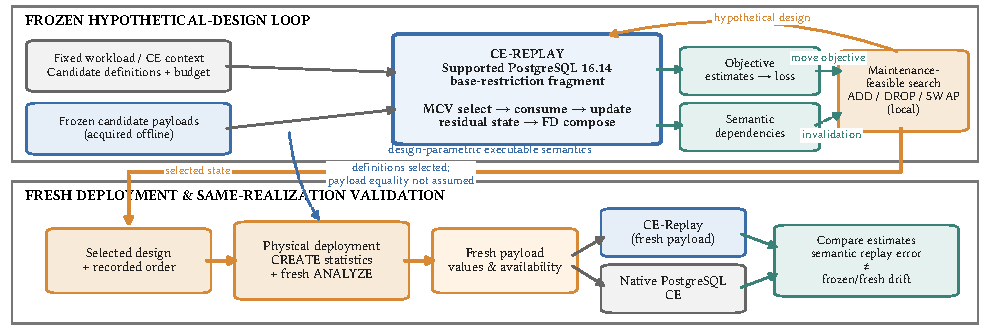
\includegraphics[width=\textwidth,height=2.20in,keepaspectratio]{figures/f1-ce-replay-architecture.pdf}
\caption{\textbf{CE-Replay physical-design pipeline.} For a supplied target workload, workload-fixed estimator context and an offline frozen candidate-payload repository specialize the supported PostgreSQL 16.14 statistics-sensitive base-restriction fragment while leaving design-dependent MCV selection, clause consumption, FD applicability, and numerical updates executable. CE-Replay exposes an objective oracle and a semantic dependency oracle to maintenance-feasible ADD/DROP/SWAP search. The selected physical state is then created with its recorded PostgreSQL realization and analyzed afresh. Fresh payloads feed both CE-Replay and native PostgreSQL for same-realization semantic validation; equality between frozen and fresh payloads is not assumed.}
\Description{Final vector figure F1; its visual content is described by the caption and repository figure plan.}
\label{fig:f1}
\end{figure*}

\subsection{What is frozen and what remains executable}

The representation has four blocks:

\begin{enumerate}
\item \textbf{Workload-fixed context:} clauses, relation cardinality, ordinary selectivities, predicate semantics, and truth retained only for later scoring.
\item \textbf{Payload and schema context:} MCV values and frequencies, base frequencies, FD degrees, semantic dimensions, key order, and payload availability.
\item \textbf{Design-dependent state:} the selected definitions and relevant physical realization, including recorded PostgreSQL precedence.
\item \textbf{Executable semantics:} applicability, GreedyCover, consumption, MCV numerical combination, FD application, and final row computation.
\end{enumerate}
Specialization fixes the first block and loads the second, while the third remains an input and the fourth executes for every hypothetical state. Freezing a winner observed under one design would violate design-parametric replay. A response table over complete designs would also discard the state transitions needed for counterfactual dependency analysis.

\subsection{Supported boundary and validation model}

The validated boundary is PostgreSQL 16.14 conjunctive base-relation restrictions with supported scalar predicates, constant \texttt{IN}/\texttt{= ANY} MCV predicates, MCV, equality-eligible FD, MCV-first composition, and relevant fixed precedence. CE-Replay does not cover joins, complete planner/path search, arbitrary expressions or operators, general Boolean trees, all statistics mechanisms, or other PostgreSQL versions.

Native instrumentation exposes the supported estimator at a raw/pre-clamp boundary. Comparisons match query, design, precedence, and payload realization, avoiding integer plan-row rounding as apparent semantic error. The native system is a semantic validation oracle; it is not invoked for every hypothetical state in the final search loop.

\subsection{Objective and dependency interfaces}

The objective oracle returns the replayed estimate and, after ground-truth scoring, the target-workload loss. It is exact only relative to the validated semantics and supplied realization. It does not predict truth.

The dependency oracle is derived from the executable state transitions rather than attached as post hoc metadata. It reports which queries, semantic dimensions, and downstream mechanisms a design move may affect, distinguishing \textbf{realized dependencies} exercised in the current trace from \textbf{structural/counterfactual dependencies} that can change a future trace even when current outputs coincide. State sufficient to continue one execution is not necessarily safe for arbitrary extension; current-output equivalence is not counterfactual-state equivalence.

\subsection{Frozen and fresh realizations}

Optimization is conditional on the frozen payload repository. Deployment invokes \texttt{ANALYZE} and creates a fresh realization whose values or availability may differ. \textbf{Semantic replay error} is the replay/native discrepancy for one matched realization. \textbf{Payload realization drift} is the difference between frozen and fresh outcomes. Figure~\ref{fig:f1} separates these quantities, and Section 7 reports them separately.

\section{Semantics-Guided Physical Design}\label{sec:6}

The optimizer is one replaceable consumer of CE-Replay's two interfaces, not the primary contribution. The implementation below tests whether those interfaces suffice for a complete maintenance-constrained search loop.

\subsection{Search policy}

The solver first builds a maintenance-feasible design by repeatedly recomputing contextual loss reduction per maintenance unit. It then enumerates all feasible ADD, DROP, and SWAP moves under fixed recorded precedence. Each round accepts the deterministic best strict improvement and terminates when none exists.

\begin{table*}[t]
\centering
\begin{minipage}{0.94\textwidth}
\begin{verbatim}
design <- empty
while a feasible candidate has positive contextual benefit per maintenance unit:
    add the deterministic best candidate and update replay state

repeat:
    best <- none
    for each feasible ADD, DROP, and SWAP:
        affected <- dependency_oracle(design, move)
        value <- objective_oracle.incremental(design, move, affected)
        best <- deterministic_best_improvement(best, value)
    if best is none or not a strict improvement:
        return design
    commit(best)
\end{verbatim}
\end{minipage}
\end{table*}

The result is locally optimal only under this audited neighborhood, payload repository, budget, and fixed precedence. Exhaustive global agreement is established only on a five-candidate Census instance and four restricted DMV instances; no approximation guarantee is claimed.

\subsection{Safe incremental evaluation}

Candidate-query incidence supplies an outer affected set. Within an affected query, the evaluator chooses the narrowest safe action: no work, a cached numerical update, local MCV control replay, FD replay after direct or upstream invalidation, or broader replay fallback. A computation is skipped only when structural/counterfactual dependencies show that the move cannot affect it.

Global graph connectivity does not invalidate this strategy. A candidate can affect few queries even when chains of shared candidates place nearly the whole workload in one connected component. Conversely, a shared maintenance budget prevents disjoint query neighborhoods from becoming completely independent optimization problems because candidates can exchange budget through SWAP moves.

Reduced semantic work is not synonymous with runtime improvement. Once control replay is avoided, numerical aggregation and move-loop overhead may dominate. Section 7 therefore reports exact trajectory preservation, replay-operation reduction, evaluator latency, and optimizer wall-clock separately.

\subsection{Deployment boundary}

After search, selected definitions are created in recorded order and analyzed afresh. Fresh payloads are passed both to CE-Replay and native PostgreSQL for same-realization validation. Candidate-payload acquisition remains an offline input boundary and is not counted as recurring deployed maintenance.

\section{Evaluation}\label{sec:7}

\subsection{Experimental Setup}

The evaluation asks four questions: whether replay matches native semantics, supports constrained design, preserves move values while reducing work, and keeps interacting mechanisms faithful after deployment. All semantic claims target PostgreSQL 16.14.

\textbf{Table~\ref{tab:t1}} establishes the complementary workload regimes used throughout the evaluation.


\begin{table*}[t]
\centering
\small
\caption{Complementary workload and candidate structure. Degree counts target queries incident to a structural-pair candidate; these workloads are not claimed to represent all database workloads.}
\label{tab:t1}
\begin{tabularx}{\textwidth}{@{}>{\raggedright\arraybackslash}X>{\raggedright\arraybackslash}X>{\raggedright\arraybackslash}X>{\raggedright\arraybackslash}X>{\raggedright\arraybackslash}X>{\raggedright\arraybackslash}X>{\raggedright\arraybackslash}X@{}}
\toprule
Workload & Queries / rows & Predicate columns / form & Pairs & Candidate degree & Incidence & Main stress \\
\midrule
Census & 468 / 2,458,285 & 68; numeric equality/range & 2,253 & Mean 4.44; max 13 & Sparse, giant component & Large universe; sparse incremental evaluation \\
DMV & 1,965 / 11,591,877 & 9; categorical equality and constant \texttt{IN}/\texttt{= ANY} & 36 & Mean 497.08; median 498; max 546 & Dense/high reuse & ScalarArray semantics; dense incremental evaluation \\
\bottomrule
\end{tabularx}
\end{table*}

Census stresses a large pair universe, mixed-mechanism selection, sparse invalidation, and realization analysis. DMV contains 1,913 IN-bearing queries and stresses bounded ScalarArray semantics, dense candidate reuse, independent maintenance calibration, and second-workload deployment. Its small candidate universe does not establish Census-scale search scalability.

Structural pairs induce mechanism-specific MCV and FD definitions. Census has 2,253 pair MCV definitions and 758 usable query-applicable FD payloads in the mixed realization. DMV has 36 pairs; its optimization realization has 36 usable MCV and 34 usable FD payloads. Baseline, optimization, and fresh DMV realizations are kept separate; absolute losses are compared only within their originating realization.

Ground-truth rows score replayed estimates using the q-error in Section 3. Two DMV queries have zero true cardinality, and the frozen positive floor makes them dominate raw aggregate DMV loss. We preserve the completed objective, use nonzero-truth loss only diagnostically, and never compare raw Census and DMV loss magnitudes.

Recurring maintenance is instantiated with mechanism-weighted object counts fitted independently to aggregate \texttt{ANALYZE} latency. \textbf{Figure~\ref{fig:f3}} uses separate workload panels because absolute costs and fitted coefficients are environment-specific.

\begin{figure*}[t]
\centering
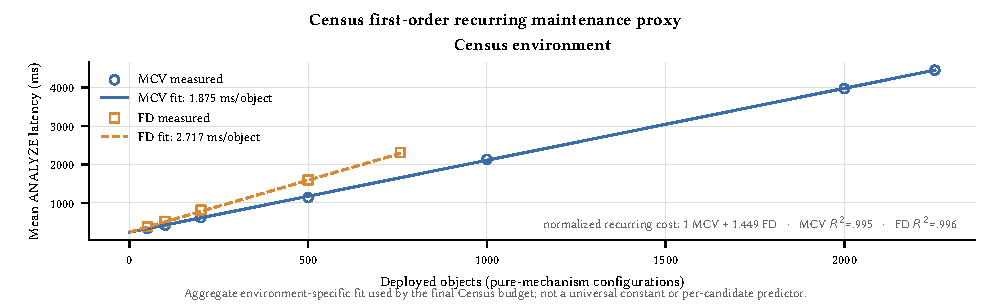
\includegraphics[width=\textwidth,height=2.05in,keepaspectratio]{figures/f3-analyze-maintenance-cost.pdf}
\caption{\textbf{Mechanism-aware recurring ANALYZE cost.} Separate workload panels relate deployed mechanism composition to aggregate \texttt{ANALYZE} latency. Census slopes are 1.874997 ms/MCV and 2.717261 ms/FD; the DMV combined model estimates 3.903845 ms/MCV and 5.907345 ms/FD. Fits and deployment errors are environment-specific, not portable PostgreSQL constants.}
\Description{Final vector figure F3; its visual content is described by the caption and repository figure plan.}
\label{fig:f3}
\end{figure*}

The controls align with those questions. Raw native comparisons test semantic fidelity; exhaustive five-candidate Census and four restricted DMV searches test small-instance optimization; complete terminal ADD/DROP/SWAP audits establish neighborhood-local termination; and incremental-versus-control trajectories test move equivalence. Deployment then evaluates fresh same-realization fidelity separately from frozen-to-fresh drift.

\subsection{RQ1 --- Does replay match native PostgreSQL?}

RQ1 asks whether CE-Replay reproduces native PostgreSQL estimates inside the supported fragment. \textbf{Table~\ref{tab:t2}} combines controlled semantic cases, real workloads, and fresh deployments.


\begin{table*}[t]
\centering
\small
\caption{Native fidelity in the supported fragment. Comparisons match query, design, precedence, and payload realization; error is relative at the raw/native cardinality boundary.}
\label{tab:t2}
\begin{tabularx}{\textwidth}{@{}>{\raggedright\arraybackslash}X>{\raggedright\arraybackslash}X>{\raggedright\arraybackslash}X>{\raggedright\arraybackslash}X>{\raggedright\arraybackslash}X@{}}
\toprule
Validation setting & Semantic fragment & Comparisons & Result & Maximum relative error \\
\midrule
Census MCV raw oracle & Scalar MCV & Four targets $\times$ 32 designs & All matched & 5.55e-16 \\
Controlled FD scenarios & FD selection, application, order & 13 scenarios & All matched & 0 \\
Synthetic ScalarArray & Constant \texttt{IN}/\texttt{= ANY} MCV & 29 cases & 29/29; scalar regression 128/128 & 4.38e-15 \\
DMV baseline realization & Real equality/IN MCV+FD & 27,510 & 27,510/27,510 & 1.40286e-14 \\
Census fresh deployment & Fresh mixed MCV+FD & 468 & 468/468 & 6.92e-16 \\
DMV fresh deployment & Fresh mixed MCV+FD & 1,965 & 1,965/1,965 & 2.43422e-14 \\
\bottomrule
\end{tabularx}
\end{table*}

Raw instrumentation removes rounded plan rows as an observation artifact. ScalarArray support retains all 128 scalar regression cases while covering the canonical DMV workload. Fresh deployment is the strongest closure because new payloads are generated: CE-Replay matches native estimates for every fresh query in both workloads.

\textbf{Answer to RQ1.} Within the explicitly supported PostgreSQL 16.14 statistics-sensitive base-restriction fragment and matched payload realization, CE-Replay matches native estimates to the reported floating-point tolerances. This result does not cover joins, full planner search, arbitrary predicates, other mechanisms, or other PostgreSQL versions.

\subsection{RQ2 --- Can replay drive resource-constrained statistics design?}

RQ2 first asks whether selection remains necessary before capacity becomes binding. \textbf{Figure~\ref{fig:f2}} answers that question by separating semantic harm from maintenance scarcity.

\begin{figure*}[t]
\centering
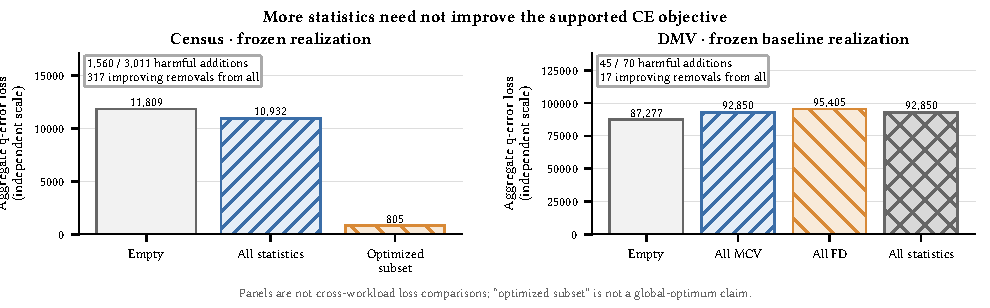
\includegraphics[width=\textwidth,height=2.05in,keepaspectratio]{figures/f2-cross-workload-nonmonotonicity.pdf}
\caption{\textbf{Cross-workload non-monotonicity.} Separate, independently scaled panels compare empty and complete states. Census has 1,560 harmful singleton additions among 3,011 candidates and 317 improving removals; DMV has 45 harmful additions among 70 usable candidates and 17 improving removals. This is contextual evidence from two frozen realizations, not a universal workload property.}
\Description{Final vector figure F2; its visual content is described by the caption and repository figure plan.}
\label{fig:f2}
\end{figure*}

In Census, empty, all-statistics, and optimized-subset losses are 11,808.960379, 10,932.295550, and 805.316472 within the shared frozen realization. In the DMV baseline realization, all-mixed equals all-MCV because MCV consumption suppresses every usable FD. These results establish semantic necessity; Figure~\ref{fig:f3} independently establishes recurring resource demand.

Having established semantic need, \textbf{Table~\ref{tab:t3}} asks what the optimizer selects under the maintenance constraint. DMV raw loss is retained for consistency but is dominated by the two zero-truth queries.


\begin{table*}[t]
\centering
\small
\caption{Maintenance-budget design outcomes. Local optimum is limited to the audited ADD/DROP/SWAP neighborhood under fixed payload and precedence. DMV [ZT] is the preserved raw objective, dominated by two zero-truth queries under the positive floor; optimization used it, while nonzero-truth loss is diagnostic only.}
\label{tab:t3}
\begin{tabularx}{\textwidth}{@{}>{\raggedright\arraybackslash}X>{\raggedright\arraybackslash}X>{\raggedright\arraybackslash}X>{\raggedright\arraybackslash}X>{\raggedright\arraybackslash}X>{\raggedright\arraybackslash}X@{}}
\toprule
Workload & Usable universe & Selected design & Budget; cost / unused & Frozen loss & Terminal audit \\
\midrule
Census & 2,253 MCV + 758 FD & 276 MCV + 7 FD & 286.144; 286.143 / 0.001 & 787.809381 & 565,031 moves; local optimum \\
DMV optimization realization & 36 MCV + 34 FD & 11 MCV + 12 FD & 43.724603; 29.158543 / 14.566060 & 7.83651388676e298 [ZT] & 47 ADD, 23 DROP, 1,081 SWAP; local optimum \\
\bottomrule
\end{tabularx}
\end{table*}

For Census, changing only the resource semantics from the earlier byte proxy to the maintenance model changes the design from 205 MCV plus 56 FD to 276 MCV plus seven FD. In the shared context, loss falls from 805.316472 to 787.809381, and all seven selected FDs are consumed. For DMV, the 50\%, 75\%, and 100\% budget levels return the same 11-MCV plus 12-FD state, leaving capacity unused because no accepted move improves the objective. Four restricted exhaustive instances recover their exact restricted optima.

\textbf{Answer to RQ2.} CE-Replay drives maintenance-constrained mixed statistics design without a learned design-to-q-error response model. The workload-scale states are audited neighborhood local optima, not global optima.

\subsection{RQ3 --- Do semantic dependencies reduce move-evaluation work?}

RQ3 asks both whether incremental evaluation preserves decisions and whether less semantic work becomes lower runtime. \textbf{Table~\ref{tab:t4}} keeps exactness, semantic/control-work reduction, and wall-clock behavior separate across sparse and dense incidence.


\begin{table*}[t]
\centering
\small
\caption{Exact incremental evaluation across incidence regimes. Semantic work and wall-clock outcomes remain separate.}
\label{tab:t4}
\begin{tabularx}{\textwidth}{@{}>{\raggedright\arraybackslash}X>{\raggedright\arraybackslash}X>{\raggedright\arraybackslash}X>{\raggedright\arraybackslash}X>{\raggedright\arraybackslash}X@{}}
\toprule
Setting & Incidence & Audited exactness & Semantic-work reduction & Wall clock \\
\midrule
Census MCV local search & Sparse; mean degree 4.44 & 5,639,186 moves; 17 accepted and final state identical & 171.31$\times$ fewer query control replays; 95.28\% no control replay & 82.422 s vs 289.013 s; 3.51$\times$ \\
Census mixed local search & Sparse; directed MCV$\rightarrow$FD & 9,107,766 moves; 19 accepted and final state identical & 95.13\% numerical-only; 154.61$\times$ control reduction & 145.68 s vs 45.05 s; 3.23$\times$ slower \\
DMV mixed optimization & Dense; mean degree 497.13 & 1,151 terminal moves; four restricted exact recoveries & 67.91\% full-workload query replay operations avoided & No comparable speedup claim \\
\bottomrule
\end{tabularx}
\end{table*}

Census contains a giant component despite sparse degree, so connected-component decomposition is ineffective. Local invalidation remains useful because a typical move touches few queries. The MCV-only evaluator preserves its complete accepted trajectory and improves measured phase time. The mixed evaluator also preserves its trajectory and sharply reduces control work, yet it is slower because numerical aggregation and Python move-loop overhead dominate. DMV shows that dependency-aware evaluation still avoids work under dense incidence, although the opportunity is smaller.

\textbf{Answer to RQ3.} Realized and structural/counterfactual dependencies enable exact audited incremental move evaluation in sparse and dense regimes. Topology controls the opportunity, and semantic-work reduction does not guarantee wall-clock improvement.

\subsection{RQ4 --- Does replay preserve interacting semantics after physical deployment?}

RQ4 asks whether replay preserves the directed MCV-to-FD interaction through complete design and physical deployment. \textbf{Figure~\ref{fig:f4}} links that mechanism to observed FD reachability.

\begin{figure*}[t]
\centering
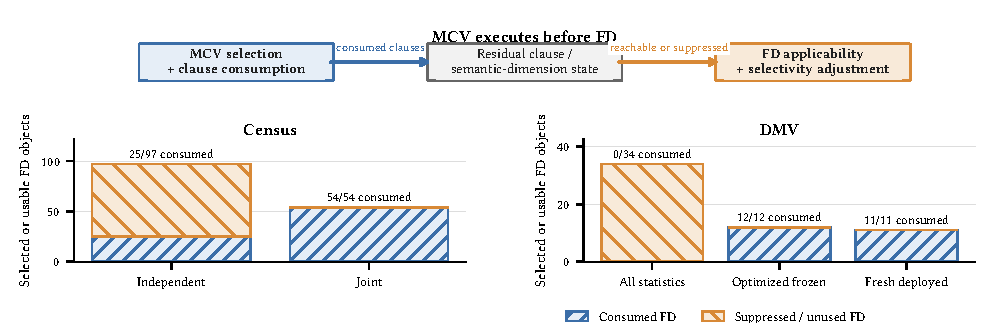
\includegraphics[width=\textwidth,height=2.15in,keepaspectratio]{figures/f4-mcv-fd-composition.pdf}
\caption{\textbf{Directed MCV-to-FD composition and FD consumption.} MCV clause consumption feeds FD residual state. Census independent optimization selects 97 FDs, 72 unused after composition; joint optimization selects 54, all consumed. DMV all-statistics consumes zero of 34 usable FDs; optimization consumes all 12 selected frozen FDs and all 11 materialized fresh FDs.}
\Description{Final vector figure F4; its visual content is described by the caption and repository figure plan.}
\label{fig:f4}
\end{figure*}

Joint Census optimization improves over independently optimized mechanisms and stops spending maintenance capacity on many suppressed FDs. DMV replicates the interaction under dense incidence. \textbf{Table~\ref{tab:t5}} then separates physical realization, fresh same-realization fidelity, and frozen-to-fresh drift.


\begin{table*}[t]
\centering
\small
\caption{Physical deployment and fresh validation. Unavailable DMV drift reflects missing frozen provenance, not assumed zero drift.}
\label{tab:t5}
\begin{tabularx}{\textwidth}{@{}>{\raggedright\arraybackslash}X>{\raggedright\arraybackslash}X>{\raggedright\arraybackslash}X>{\raggedright\arraybackslash}X>{\raggedright\arraybackslash}X>{\raggedright\arraybackslash}X@{}}
\toprule
Workload & Selected / fresh materialized & FD consumption & Fresh replay/native; max relative error & Frozen$\rightarrow$fresh drift & Cost error \\
\midrule
Census & 276 MCV + 7 FD; 276/276 MCV, 7/7 FD & 7/7 & 811.553725 / 811.553725; 468/468; 6.92e-16 & 787.809381 $\rightarrow$ 811.553725; +3.0140\% & 7.20\% \\
DMV & 11 MCV + 12 FD; 11/11 MCV, 11/12 FD & 11/11 materialized; 389 queries & 1,965/1,965; aggregate equal; 2.43422e-14 & Unavailable: frozen per-query provenance not persisted & 21.4295\% \\
\bottomrule
\end{tabularx}
\end{table*}

For Census, all objects materialize and consume. Across 30 repeated \texttt{ANALYZE} realizations, 14,040/14,040 replay/native comparisons match while payloads and objective values vary. This demonstrates same-realization fidelity under payload variation, not stability of design rankings. For DMV, one selected FD payload does not materialize, but every materialized FD consumes and all fresh queries match native. The original optimization artifact lacks sufficient frozen per-query state for a paired DMV drift distribution; this provenance gap does not invalidate fresh semantic fidelity or physical composition.

\textbf{Answer to RQ4.} CE-Replay composes directed MCV and FD semantics and remains faithful after fresh physical deployment on both workloads. Fresh realization can change values and availability, so semantic replay error and payload realization drift must remain separate.

\section{Discussion and Limitations}\label{sec:8}

\subsection{Statistics as semantic physical design}

Extended statistics change the optimizer's information state, and their utility depends on native selection, consumption, and mechanism composition---not only on captured correlation. The cross-workload non-monotonicity evidence therefore justifies selection independently of scarcity, while recurring collection work supplies a separate resource justification. A loose budget removes neither contextual harm nor the need to choose.

\subsection{CE-Replay as an optimization representation}

CE-Replay's value is representational rather than merely computational. Configuration-parametric representation and dependency-aware recomputation are established principles; CE-Replay instead represents statistics-sensitive estimator state transitions that provide both the hypothetical objective and the statistics-semantic information needed to invalidate that objective safely after a move. Within the supported fragment, native semantics supply the design response without a separately learned subset-to-error model; outside that boundary, approximate or learned components may still be useful.

Execution-sufficient state is not necessarily counterfactual-safe state. A currently unused object may change a future winner, and numerically equal current states can diverge after an extension. This is why structural/counterfactual dependencies supplement the realized trace.

\subsection{Locality without decomposition}

Census rejects a tempting but incorrect shortcut. Its graph is globally connected and tested factorization does not yield independent subproblems, yet sparse candidate degree permits local recomputation. The semantic representation reduces exact move-evaluation work; it does not decompose away the global budget or combinatorial search.

The mixed-evaluator slowdown identifies the limit of that opportunity. Once semantic control replay becomes rare, numerical aggregation and implementation overhead dominate; less replay work does not guarantee end-to-end acceleration. DMV confirms correctness in a dense regime while exposing less locality, but two workloads do not define a universal scaling law.

\subsection{Maintenance cost and semantic utility}

Payload bytes were an early controlled proxy. The final resource is recurring maintenance, instantiated through mechanism-weighted object counts calibrated from aggregate \texttt{ANALYZE} latency. Coefficients differ across Census and DMV and deployment prediction errors remain visible. The model is a first-order environment-specific resource proxy, not a PostgreSQL constant or a per-object latency predictor.

Changing resource semantics changes the physical-design problem: on Census it materially changes composition and frozen loss. A budget is a capacity constraint, not a target; a local optimum may leave capacity unused when no feasible neighborhood move improves the contextual objective.

\subsection{Frozen hypothetical state and fresh realization}

The optimizer is conditional on a frozen payload repository, while deployment generates a fresh realization. Replay/native fidelity within one realization and frozen-to-fresh drift answer different questions. Repeated Census \texttt{ANALYZE} demonstrates payload and objective variability without semantic mismatch. It does not establish frequent design-ranking reversal or regret; that would require paired multi-design realizations.

Future objectives could optimize expected, risk-sensitive, or worst-case loss over realizations. Efficient acquisition of hypothetical candidate payloads is another open systems problem. Just-in-time, piggyback, and modern incremental statistics maintenance demonstrate complementary ways to reduce collection or refresh work ~\cite{elhelw2007jits,zhu2004piggyback,pfeil2026redshift}. CE-Replay does not implement those techniques: its offline acquisition boundary is distinct from the recurring maintenance cost of the selected deployment.

\subsection{Extending CE-Replay}

The implementation is source-informed and mechanism-specific rather than an automatic compiler. Supporting another predicate family, mechanism, version, or DBMS requires extracting applicability and control rules, defining payload schemas, implementing state transitions, validating native behavior, and exposing dependencies. The ScalarArray extension demonstrates this deliberate process. MCV-to-FD composition suggests an architectural principle---mechanisms should expose explicit state inputs, outputs, and dependency boundaries---but the principle has not been validated across DBMSs.

PostgreSQL-specific elements include GreedyCover, OID precedence, payload formats, MCV-to-FD ordering, and \texttt{ANALYZE} realization behavior. The contribution is the bounded executable estimator-semantic representation and its validated interfaces; workload specialization, configuration parametrization, dependency-aware recomputation, and maintenance-constrained design are established foundations.

\subsection{Limitations}

The validated semantic scope is PostgreSQL 16.14 conjunctive base-relation restrictions with supported scalar and constant \texttt{IN}/\texttt{= ANY} predicates, MCV, FD, and their directed composition. It excludes joins, planner/path search, arbitrary expressions/operators or Boolean trees, other mechanisms, and other versions. The semantics were manually engineered and validated, not automatically compiled.

Optimization assumes an offline frozen payload repository and returns an ADD/DROP/SWAP neighborhood local optimum under fixed precedence; it has no full-instance global or approximation guarantee. The maintenance model is environment-specific and first-order. The objective is q-error, not plan quality, latency, throughput, or a causal runtime improvement.

Fresh \texttt{ANALYZE} can change payloads or availability, and the optimizer is not realization-robust. DMV raw aggregate loss is dominated by two zero-truth queries under the preserved positive floor. DMV also lacks sufficient frozen per-query provenance for complete paired drift reconstruction, although fresh fidelity and composition remain supported.

Finally, Census and DMV provide complementary sparse and dense evidence but do not establish universal workload generality. The target workload is supplied; unseen-workload generalization is outside the core problem.

\section{Related Work}\label{sec:9}

\subsection{Statistics management and multivariate-statistics discovery}

Automatic statistics management predates CE-Replay. Chaudhuri and Narasayya select optimizer-relevant statistics, explicitly note dependencies among statistics, and show in MNSA/D that a statistic irrelevant under one set can matter after another statistic is added ~\cite{chaudhuri2001statistics}. CORDS discovers correlations and soft functional dependencies for joint statistics, while JITS selects and collects query-specific statistics using sensitivity and prior information ~\cite{ilyas2004cords,elhelw2007jits}. Thus workload-aware selection, contextual statistics relevance, correlation discovery, and selective acquisition are established.

Their MNSA analysis uses a cost-monotonicity assumption over predicate selectivities, while also acknowledging pathological violations in which adding a histogram can worsen the chosen plan ~\cite{chaudhuri2001statistics}. Our non-monotonicity evidence concerns PostgreSQL q-error under physically realized extended-statistics objects; it is systematic evidence for semantics-aware selection in this mechanism and setting, not a claim that harmful additions are historically new.

CE-Replay does not contribute candidate discovery, acquisition, or statistics interaction in general. Given definitions and frozen payloads, it represents the native estimator transitions producing those interactions---applicability, precedence, clause consumption, numerical updates, and downstream reachability---and uses them for hypothetical CE and move invalidation.

Statistics collection and refresh are also established concerns. Piggyback collection gathers statistics during query execution ~\cite{zhu2004piggyback}, while JITS considers materialization and maintenance of selectively collected statistics ~\cite{elhelw2007jits}. Recent Redshift work updates optimizer statistics incrementally from modified data rather than repeatedly scanning full tables ~\cite{pfeil2026redshift}. These techniques ask how to acquire or refresh a chosen statistical state efficiently. CE-Replay asks which state to choose under a recurring maintenance constraint; combining the two directions is future systems work.

\subsection{What-if and configuration-parametric physical design}

Hypothetical evaluation, constrained design, and contextual design-object interaction are established foundations. AutoAdmin evaluates hypothetical indexes without materializing every configuration; constrained tuning optimizes under storage and richer constraints; and Index Interactions formalizes configuration-dependent positive and negative index interactions, including objects that become useful together ~\cite{chaudhuri1998whatif,bruno2008constrained,schnaitter2009interactions}. CE-Replay claims none of these general principles.

INUM reuses optimizer-derived template plans while plugging in access costs for each index design ~\cite{papadomanolakis2007inum}. C-PQO specializes optimizer computation into a compact MEMO/APR representation, retaining alternatives needed to produce plans for arbitrary configurations ~\cite{bruno2008cpqo}. They establish reusable configuration-parametric optimizer representations and latent configuration alternatives, not just final-plan caching.

The distinction is the represented computation and the interface it exposes. INUM and C-PQO represent optimizer plan/cost behavior over hypothetical physical-design configurations. CE-Replay specializes the supported statistics-sensitive estimator computation itself, leaving applicability, winner selection, clause consumption, payload-dependent numerical updates, and downstream mechanism reachability executable. Those state transitions expose the statistics-semantic dependencies needed both to evaluate the CE objective and to invalidate incremental statistics-design moves safely. This is not a claim that prior physical-design tools are black boxes, lack response reuse, or cannot expose dependencies; the methodological point is that this represented computation supplies the dependency structure required by the present statistics-design problem.

\subsection{Incremental optimization}

Dependency tracking and exact incremental recomputation are established principles. Incremental query re-optimization retains optimizer search/pruning state, propagates changed cardinality or cost information, and can rederive pruned alternatives while matching full reoptimization ~\cite{liu2016incremental}. CE-Replay's narrower contribution is to identify and expose the estimator-semantic state affected by a statistics-design move---including precedence, consumption, and downstream reachability---before optimizer search. We therefore use \textbf{semantic dependency oracle} as a domain-specific interface, not a claim to generic incremental computation.

\subsection{Cardinality estimation}

Learned and data-driven CE systems construct alternative estimation models. MSCN learns from query features and executed-query cardinalities ~\cite{kipf2019learned}; DeepDB learns a data-driven probabilistic model rather than requiring executed-query workload training ~\cite{hilprecht2020deepdb}; FactorJoin combines learned single-table conditional distributions through a factor graph for join estimation ~\cite{wu2023factorjoin}. This variety prevents a simple learning-versus-no-learning dichotomy.

CE-Replay does not learn a replacement cardinality estimator or a surrogate mapping from statistics designs to q-error. It executes the supported statistics-sensitive semantics of PostgreSQL's native estimator while varying the physical statistics state. PostgreSQL documentation and source define the native MCV/FD mechanisms ~\cite{postgresql16docs,postgresql16source}; this paper contributes their bounded extraction, executable encoding, composition, and validation for physical-design evaluation, not the mechanisms themselves.

\subsection{Positioning of CE-Replay}

Prior work establishes statistics dependencies and contextual interactions among design objects, hypothetical and configuration-parametric optimizer evaluation, and dependency-aware exact recomputation. CE-Replay's bounded systems specialization is to preserve the supported native statistics-estimator state transitions as executable design parameters, using that state for both workload CE evaluation and statistics-semantic, counterfactual-safe move invalidation.

This positioning is deliberately bounded. The literature categories overlap, and the current search does not justify a priority claim. CE-Replay is neither a complete advisor pipeline nor a full PostgreSQL estimator: candidate-payload acquisition remains external, search remains replaceable and neighborhood-local, and semantic coverage remains the validated PostgreSQL 16.14 fragment.

\section{Conclusion}\label{sec:10}

This paper studies extended-statistics design for a supplied target workload under a recurring maintenance constraint. Selection is necessary both because deployed objects consume maintenance capacity and because native estimator control makes candidate utility contextual and non-monotone.

CE-Replay exposes the supported statistics-sensitive semantics as a workload-specialized, design-parametric executable representation. Workload-fixed context is specialized, while applicability, winner selection, clause consumption, MCV-to-FD composition, and numerical payload behavior remain executable. The resulting objective and dependency oracles allow a replaceable optimizer to evaluate hypothetical states and safely restrict recomputation.

For the supported PostgreSQL 16.14 base-restriction fragment, Census and DMV establish same-realization fidelity within floating-point tolerance, maintenance-aware mixed designs, audited incremental equivalence in sparse and dense regimes, and fresh physical deployment. The negative results delimit the method: global connectivity need not eliminate local invalidation, less semantic replay does not guarantee faster optimization, and fresh payload drift remains distinct from semantic replay error.

The current results remain conditional on a supplied workload, a frozen payload repository, manually supported MCV+FD semantics, and neighborhood-local search. Extending executable semantic representations to broader CE mechanisms, cheaper payload acquisition, realization-aware objectives, and additional DBMSs offers a path toward physical-design tools that use native estimator behavior as both an objective evaluator and a source of optimization structure.

\section*{Artifact and Reproducibility Statement}\label{sec:artifact}

The public repository contains experiment scripts, frozen results, and claim/evidence audits. The immutable \texttt{research-freeze-v0} tag identifies the experimental baseline used by this draft; later commits contain paper-construction artifacts. The reproducibility index maps each main claim to its scripts and outputs. No archival DOI is claimed in this draft.
\phantomsection
\label{references-start}
\bibliographystyle{ACM-Reference-Format}
\bibliography{paper}
\end{document}
